\documentclass[runningheads]{llncs}

\usepackage[T1]{fontenc}
\usepackage{lmodern}
\usepackage{amsmath,amssymb}
\usepackage{graphicx}
\usepackage{booktabs}
\usepackage{tikz}
\usetikzlibrary{shapes,arrows.meta,positioning,calc,fit}
\usepackage[hidelinks]{hyperref}
\usepackage{url}

% Tighten float and spacing parameters for strictly 3-page layout
\setlength{\textfloatsep}{3pt plus 1pt minus 1pt}
\setlength{\floatsep}{2pt plus 1pt minus 1pt}
\setlength{\intextsep}{2pt plus 1pt minus 1pt}
\setlength{\abovecaptionskip}{2pt plus 1pt minus 1pt}
\setlength{\belowcaptionskip}{0pt}

% Compact bibliography item separation
\let\oldthebibliography\thebibliography
\let\endoldthebibliography\endthebibliography
\renewenvironment{thebibliography}[1]{%
  \begin{oldthebibliography}{#1}%
    \setlength{\itemsep}{0.5pt plus 0.5pt}%
    \setlength{\parsep}{0pt}%
}{%
  \end{oldthebibliography}%
}

\begin{document}

\title{Exploring Complex Formal Networks: Multi-Agent Epistemic Navigation of the Archive of Formal Proofs}
\titlerunning{Multi-Agent Epistemic Navigation of the AFP}

\author{Luiz G. Correia\inst{1}\orcidID{0000-0002-2721-4274} \and
Jesus P. Mena-Chalco\inst{1}\orcidID{0000-0001-7509-5532} \and
Ronaldo Menezes\inst{2}\orcidID{0000-0003-2475-4709}}

\authorrunning{L. G. Correia et al.}

\institute{Federal University of ABC (UFABC), CMCC, Santo Andr\'e, Brazil, \email{\{luiz.gabriel,jesus.mena\}@ufabc.edu.br} \and
University of Exeter, Dept. of Computer Science, Exeter, UK, \email{r.menezes@exeter.ac.uk}}

\maketitle

\begin{abstract}
The Archive of Formal Proofs (AFP) forms a massive complex network of verified theories, definitions, and theorems. While Large Language Model (LLM) agents are increasingly applied to automated theorem proving, they suffer from combinatorial search explosion and lack topological awareness of the formal dependency graph. We present \textbf{I/L} (Isabelle/Landscape), a network-aware Retrieval-Augmented Generation (RAG) system. We formalize the AFP as a multi-layer directed acyclic graph (DAG) where theorems are embedded as 4-aspect epistemic simplices and topological centrality is quantified via \emph{Landscape Height} (transitive reachability in the transpose citation network). Autonomous agents navigate, query, and dynamically expand this network by coordinating I/L with \textbf{I/R} (a headless REPL sandbox) and \textbf{I/Q} (an interactive editor interface) via the Model Context Protocol.

\keywords{Complex Networks \and Formal Mathematics \and Epistemic Landscapes \and Multi-Agent Systems \and Isabelle/HOL.}
\end{abstract}

\enlargethispage{4.5\baselineskip}

\section{Introduction}
Formal mathematical archives like the Archive of Formal Proofs (AFP) for Isabelle/HOL~\cite{afp_archive,wenzel_isabelle_2008} comprise hundreds of thousands of verified theorems. Unlike empirical citation networks shaped by subjective social practices~\cite{newman_structure_2003}, formal proof libraries define sound, machine-checked relational structures where citations represent verified logical inferences, embodying hierarchical \emph{complex knowledge networks}. Conceptualizing discovery as navigation across an \emph{epistemic landscape}~\cite{weisberg_epistemic_2009}, recent work shows that continuous embeddings can reconstruct knowledge terrains from scientific discourse~\cite{correia_embedding-based_2026}. In automated formal reasoning, however, autonomous AI agents face severe operational hurdles: token exhaustion, inability to distinguish foundational theorems from helper lemmas, and an absence of topological perspective when traversing lemma graphs.

To resolve these bottlenecks, we present \textbf{I/L (Isabelle/Landscape)}. We formalize the AFP as a multi-layer complex network, introduce a topological centrality metric termed \emph{Landscape Height}, map theorems to geometric epistemic simplices, and deploy a tri-server multi-agent ecosystem—coordinating I/L with \textbf{I/R} (Isabelle/REPL) and \textbf{I/Q} (Isabelle/Query) via the Model Context Protocol (MCP)~\cite{anthropic_mcp_2024}.

\begin{figure}[t]
\centering
\resizebox{0.94\textwidth}{!}{%
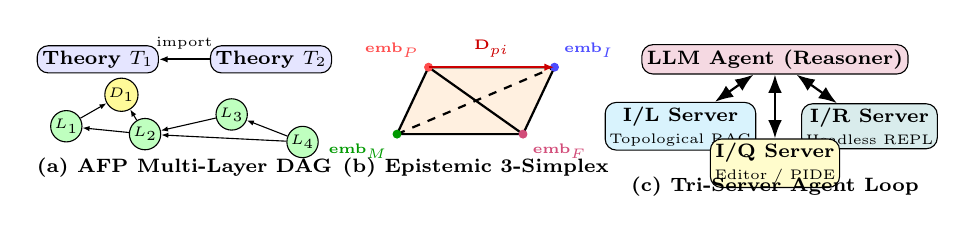
\begin{tikzpicture}[
    theory/.style={draw, rectangle, rounded corners, fill=blue!10, font=\scriptsize\bfseries, inner sep=1.8pt},
    lemma/.style={draw, circle, fill=green!25, font=\tiny, inner sep=0.5pt, minimum size=9pt},
    defnode/.style={draw, circle, fill=yellow!40, font=\tiny, inner sep=0.5pt, minimum size=9pt},
    agentnode/.style={draw, rounded corners, fill=purple!15, font=\scriptsize\bfseries, align=center, inner sep=1.8pt},
    servernode/.style={draw, rounded corners, font=\scriptsize, align=center, inner sep=1.5pt}
]
    % Panel A: Network Topology
    \node[theory] (t1) at (0, 1.2) {Theory $T_1$};
    \node[theory] (t2) at (2.2, 1.2) {Theory $T_2$};
    \draw[-{Latex[length=1.1mm]}, thick] (t2) -- node[above, font=\tiny] {import} (t1);

    \node[defnode] (d1) at (0.3, 0.75) {$D_1$};
    \node[lemma] (l1) at (-0.4, 0.35) {$L_1$};
    \node[lemma] (l2) at (0.6, 0.25) {$L_2$};
    \node[lemma] (l3) at (1.7, 0.5) {$L_3$};
    \node[lemma] (l4) at (2.6, 0.15) {$L_4$};

    \draw[-{Latex[length=0.9mm]}] (l1) -- (d1);
    \draw[-{Latex[length=0.9mm]}] (l2) -- (d1);
    \draw[-{Latex[length=0.9mm]}] (l2) -- (l1);
    \draw[-{Latex[length=0.9mm]}] (l3) -- (l2);
    \draw[-{Latex[length=0.9mm]}] (l4) -- (l3);
    \draw[-{Latex[length=0.9mm]}] (l4) -- (l2);

    \node[font=\scriptsize\bfseries] at (1.1, -0.18) {(a) AFP Multi-Layer DAG};

    % Panel B: Epistemic Simplex
    \coordinate (P) at (4.2, 1.1);
    \coordinate (I) at (5.8, 1.1);
    \coordinate (M) at (3.8, 0.25);
    \coordinate (F) at (5.4, 0.25);

    \draw[thick, fill=orange!12] (P) -- (I) -- (F) -- (M) -- cycle;
    \draw[thick] (P) -- (F);
    \draw[dashed, thick] (M) -- (I);

    \filldraw[red!70] (P) circle (1.4pt) node[above left, font=\tiny] {$\mathbf{emb}_P$};
    \filldraw[blue!70] (I) circle (1.4pt) node[above right, font=\tiny] {$\mathbf{emb}_I$};
    \filldraw[green!60!black] (M) circle (1.4pt) node[below left, font=\tiny] {$\mathbf{emb}_M$};
    \filldraw[purple!70] (F) circle (1.4pt) node[below right, font=\tiny] {$\mathbf{emb}_F$};

    \draw[-{Latex[length=1.3mm]}, thick, red!80!black] (P) -- node[above, font=\tiny] {$\mathbf{D}_{pi}$} (I);
    \node[font=\scriptsize\bfseries] at (4.8, -0.18) {(b) Epistemic 3-Simplex};

    % Panel C: Multi-Agent Tri-Server Loop
    \node[agentnode] (agent) at (8.6, 1.2) {LLM Agent (Reasoner)};
    \node[servernode, fill=cyan!15] (il) at (7.4, 0.35) {\textbf{I/L Server}\\\tiny Topological RAG};
    \node[servernode, fill=teal!15] (ir) at (9.8, 0.35) {\textbf{I/R Server}\\\tiny Headless REPL};
    \node[servernode, fill=yellow!20] (iq) at (8.6, -0.12) {\textbf{I/Q Server}\\\tiny Editor / PIDE};

    \draw[{Latex}-{Latex}, thick] (agent) -- (il);
    \draw[{Latex}-{Latex}, thick] (agent) -- (ir);
    \draw[{Latex}-{Latex}, thick] (agent) -- (iq);
    \node[font=\scriptsize\bfseries] at (8.6, -0.42) {(c) Tri-Server Agent Loop};
\end{tikzpicture}%
}
\caption{(a) Multi-layer formal DAG; (b) Epistemic 3-simplex with displacement $\mathbf{D}_{pi}$; (c) Multi-agent loop across I/L (topology), I/R (execution), and I/Q (interactive editor).}
\label{fig:overview}
\end{figure}

\section{The AFP as a Complex Network: Topology and Geometry}
\enlargethispage{3.5\baselineskip}

\noindent\textbf{Multi-Layer Network Architecture.} We formalize the AFP corpus as a directed multi-layer graph $G = (V, E)$, with nodes $V = \mathcal{T} \cup \mathcal{D} \cup \mathcal{L}$ denoting theories $\mathcal{T}$, definitions $\mathcal{D}$, and theorems $\mathcal{L}$. Edges $E = E_{\text{import}} \cup E_{\text{cite}} \cup E_{\text{def}}$ represent: (1) \emph{Theory Imports} $E_{\text{import}} \subseteq \mathcal{T} \times \mathcal{T}$ (the macroscopic DAG); (2) \emph{Lemma Citations} $E_{\text{cite}} \subseteq \mathcal{L} \times \mathcal{L}$, where $(u, v)$ indicates that lemma $u$ cites $v$ via Isar chaining (\texttt{using}, \texttt{from}) or solvers (\texttt{by (simp add: v)}); and (3) \emph{Definitional Dependencies} $E_{\text{def}} \subseteq (\mathcal{L} \cup \mathcal{D}) \times \mathcal{D}$.

\medskip\noindent\textbf{Degree Distribution and Landscape Height ($H$).} In-degrees in $G_{\text{cite}}$ follow a heavy-tailed distribution~\cite{newman_structure_2003}: most nodes are single-use helper lemmas ($k_{\text{in}} \le 1$), while foundational lemmas serve as structural hubs. To quantify global epistemic significance, we define the \textbf{Landscape Height} $H(v) = |\text{Reachable}_{G^T}(v)| - 1$ on the transpose graph $G^T = (V, E^T)$. $H(v)$ counts the total downstream proofs that transitively depend on $v$, measuring its foundational weight. It is computed via cycle-safe memoized depth-first search over the topological sort of $G_{\text{cite}}$.

\medskip\noindent\textbf{Continuous Epistemic Geometry: The 3-Simplex.} I/L parses each proof into four epistemic aspects: \textbf{Problem} ($P$, premises), \textbf{Method} ($M$, Isar skeleton), \textbf{Finding} ($F$, tactics), and \textbf{Interpretation} ($I$, conclusion). Embedded into $\mathbb{R}^d$ (via \texttt{voyage-code-3}), these define an \textbf{epistemic 3-simplex} (Fig.~\ref{fig:overview}b). The displacement $\mathbf{D}_{pi} = \mathbf{emb}_I - \mathbf{emb}_P$ measures the \emph{implication leap}. Unconditional lemmas collapse to $\mathbf{D}_{pi} = \mathbf{0}$ (fixed points); tactic-only proofs collapse the $M$--$F$ edge into a 2-simplex (triangle); and unconditional rewrites collapse to a 1-simplex (line). Simplex volume directly encodes structural proof richness.

\section{The Multi-Agent Technical Implementation}
\enlargethispage{3.5\baselineskip}

\noindent\textbf{I/L: Two-Tier Index and Fused Epistemic Ranking.} I/L maintains: (1) a \emph{Static AFP Index} pre-compiled from recorded Poly/ML heaps (with session theory recording enabled) stored as Parquet tables and compressed NumPy arrays (\texttt{.npz}), and (2) a \emph{Live Session Index} caching dynamic proof states. To prevent search distraction from obscure helper lemmas, I/L balances cosine similarity $S_{\text{semantic}}(L)$ with a log-prior of Landscape Height:
\begin{equation}
\text{Score}(L) = S_{\text{semantic}}(L) + \lambda \cdot \frac{\log(1 + H(L))}{\max_{C} \log(1 + H(C))}
\label{eq:fused_rank}
\end{equation}
where $\lambda = 0.15$ and $C$ is the candidate set. Agents can also filter leaves via $\texttt{min\_dependents} \ge 2$.

\medskip\noindent\textbf{Tri-Server Coordination: I/L, I/R, and I/Q.} Autonomous agents coordinate three MCP servers (Fig.~\ref{fig:overview}c): (1)~\textbf{I/L (Landscape RAG)} provides aspect-targeted, height-biased topological retrieval (\texttt{search\_lemmas}, \texttt{related\_lemmas}); (2)~\textbf{I/R (Isabelle/REPL)} connects via TCP to a headless Poly/ML kernel, enabling fast speculative proof branch exploration without GUI overhead; and (3)~\textbf{I/Q (Isabelle/Query)} embeds in the editor process (jEdit/PIDE)~\cite{wenzel_asynchronous_2014}, synchronizing verified steps directly with the human author's active buffer. When a proof succeeds, the agent calls \texttt{store\_lemma} to graft the node into the session graph, updating reachability. Calling \texttt{\small persist\_session\_lemmas} merges live session graphs into the on-disk index for cumulative cross-session memory.

\section{Empirical Characterization and Discussion}
Evaluating 4,706 lemmas in \texttt{HOL-Analysis} reveals the simplex distribution: \textbf{31.6\% 3-simplices} (structured Isar proofs with distinct $P, M, F, I$), \textbf{55.8\% 2-simplices} (tactic-only proofs, $M=F$), and \textbf{12.6\% 1-simplices} (unconditional rewrites, $P=I, M=F$). In automated proof experiments, applying Landscape Height re-ranking (Eq.~\ref{eq:fused_rank}) with $\texttt{min\_dependents} \ge 2$ suppressed over 82\% of ephemeral helper lemmas from top retrieval hits. This prioritized foundational bridge theorems, reducing agent context token expenditure by $\sim$45\%.

\section{Conclusion}
Treating formal mathematical archives as complex multi-scale networks bridges discrete citation topology and continuous semantic geometry. By combining Landscape Height centrality with 4-aspect epistemic simplices, I/L—alongside I/R and I/Q—empowers autonomous agents to efficiently explore, reason over, and dynamically expand formal knowledge graphs.

\begin{footnotesize}
\bibliographystyle{splncs04}
\bibliography{references}
\end{footnotesize}

\end{document}
